\documentclass[main]{subfiles}


\title[AutoML: Introduction]{AutoML Motivation}
\subtitle{Why is Machine Learning not Easy?}
\author[Marius Lindauer]{Marius Lindauer}
\date{}

\titlebackground*{images/AutoML_AutoDL}

%\institute{}
%\date{}

\begin{document}
	
	\maketitle
	

%----------------------------------------------------------------------
%----------------------------------------------------------------------
\begin{frame}[c]{Machine Learning}

\centering
\textit{``Machine learning is the science of getting computers to act\\
 without being explicitly programmed.''}\\[2em]

\hfill by Andrew Ng (inspired by Arthur Samuel?)

\end{frame}
%-----------------------------------------------------------------------
%----------------------------------------------------------------------
\begin{frame}[c]{Without Being Explicitly Programmed?}

\textcolor{ForestGreen}{Yes}
\begin{itemize}
    \item[$\to$] Machine learning models can be trained for different datasets and tasks using the same code base
\end{itemize}

\bigskip

\pause

\textcolor{red}{No?}
For different given datasets and tasks, we achieve the best performance by adapting
\begin{itemize}
    \item[$\to$] Hyperparameters for training (incl. pre-training and fine-tuning) such as learning rate, batch sizes or regularization
    \pause
    \item[$\to$] The model, such as
    \begin{itemize}
        \item Choosing the correct model class (e.g., XGBoost vs DNNs)
        \item Architecture of a deep neural network (e.g., size, operators, connections)
        \item Usage-specific changes (e.g., tokenization, prompt engineering, temperature)
    \end{itemize}
    \pause
    \item[$\to$] preprocessing of your data, such as data filtering, data normalization or data augmentation
\end{itemize}

\end{frame}
%-----------------------------------------------------------------------
%----------------------------------------------------------------------
\begin{frame}[c]{PyTorch Documentation of SGD}


\begin{columns}

\column{0.5\textwidth}

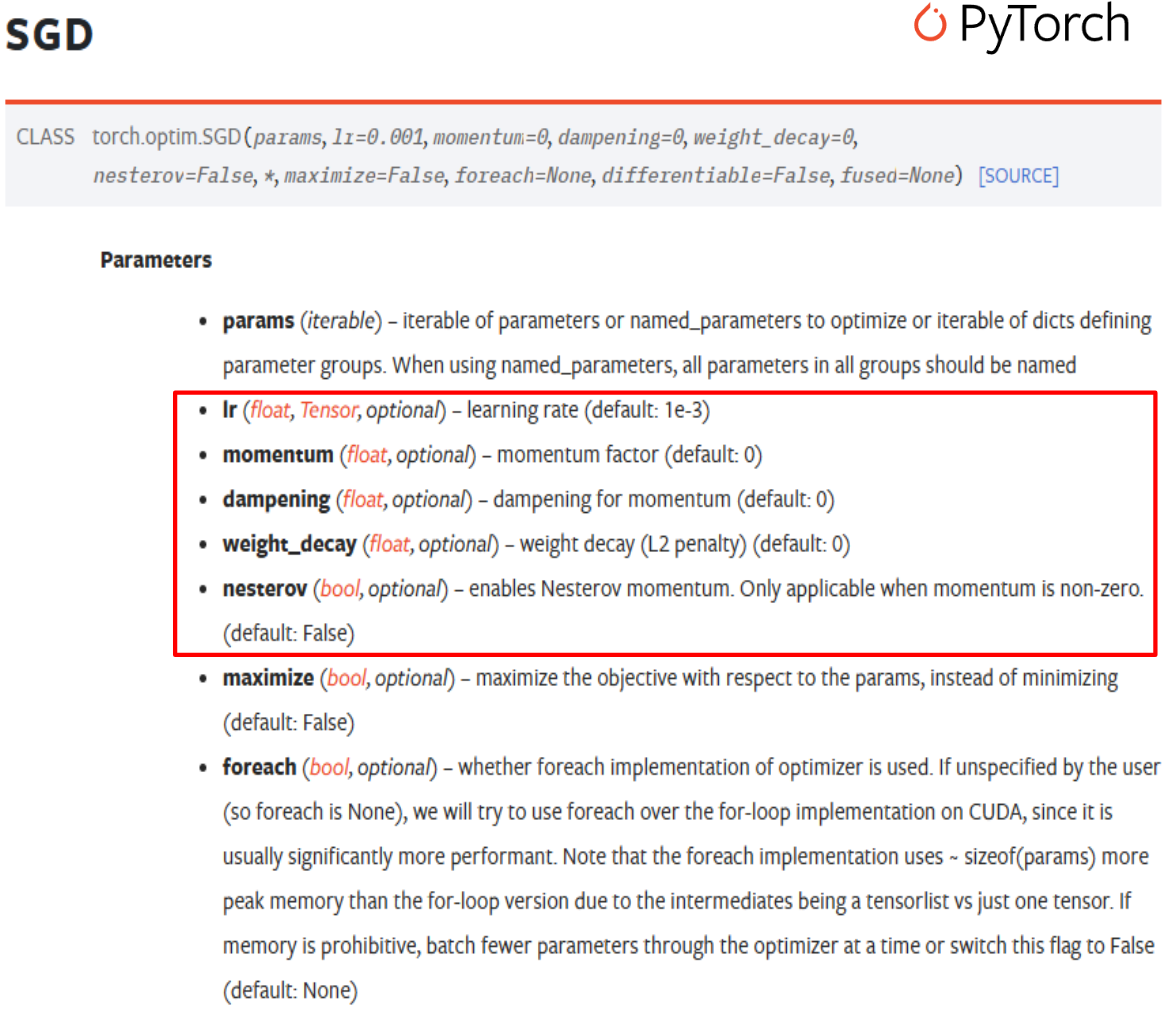
\includegraphics[width=1.0\textwidth]{images/sgd.png}

\column{0.5\textwidth}

\begin{itemize}
    \item Even a simple stochastic gradient descent -- the most basic training optimizer for DNNs, has 5 hyperparameters in PyTorch's implementation
    \item If you consider all other magic numbers -- sometimes hidden in packages you are using -- you can easily go up to 30 and more hyperparameters
    \item If you choose the wrong hyperparameter settings, your training success can suffer or completely fail
\end{itemize}
    
\end{columns}

\end{frame}
%-----------------------------------------------------------------------
% TODO: It would be nice to have a graphic showing the impact of the learning rate 
%----------------------------------------------------------------------
\begin{frame}[c]{ResNet Implementation \liturl{Digital Ocean}{https://www.digitalocean.com/community/tutorials/writing-resnet-from-scratch-in-pytorch}}


\begin{columns}

\column{0.5\textwidth}

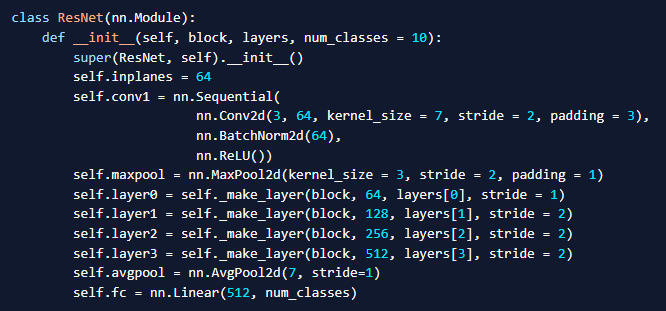
\includegraphics[width=1.0\textwidth]{images/resnet.png}

\column{0.5\textwidth}

\begin{itemize}
    \item Even a simple ResNet has many magic numbers, e.g., number of channels, kernel size, padding, stride, number of res-blocks, and so on
    \item The ResNet architecture is well defined, but if you need to find a variation of it, you are facing the question of which operators to connect how?
    \item The correct architecture of your network can decide whether you will obtain a good model or not
\end{itemize}
    
\end{columns}

\end{frame}
%-----------------------------------------------------------------------
%----------------------------------------------------------------------
\begin{frame}[c]{Data Augmentation \liturl{PyTorch Docu}{https://docs.pytorch.org/vision/main/transforms.html}}


\begin{columns}

\column{0.5\textwidth}

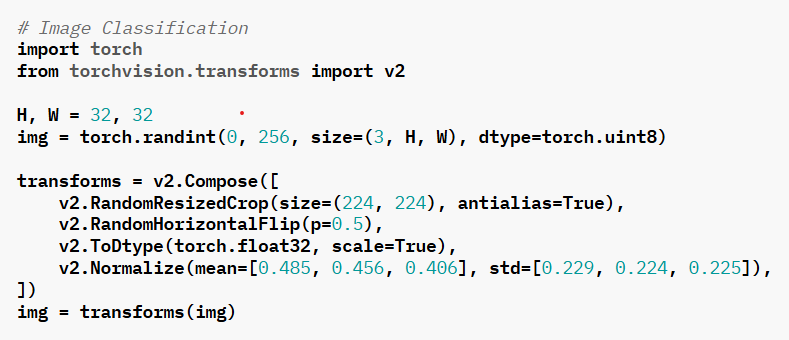
\includegraphics[width=1.0\textwidth]{images/dataaugment.png}

\column{0.5\textwidth}

\begin{itemize}
    \item Data Augmentation strategies can be important to increase the dataset size and to help with transformation- invariant predictions
    \item However, it depends on your task what kind of transformations are reasonable and required
\end{itemize}
    
\end{columns}

\end{frame}
%-----------------------------------------------------------------------
%----------------------------------------------------------------------
\begin{frame}[c]{Fine-Tuning of LLMs \liturl{PyTorch Doc}{https://docs.pytorch.org/torchtune/0.4/tutorials/lora_finetune.html}}


\begin{columns}

\column{0.5\textwidth}

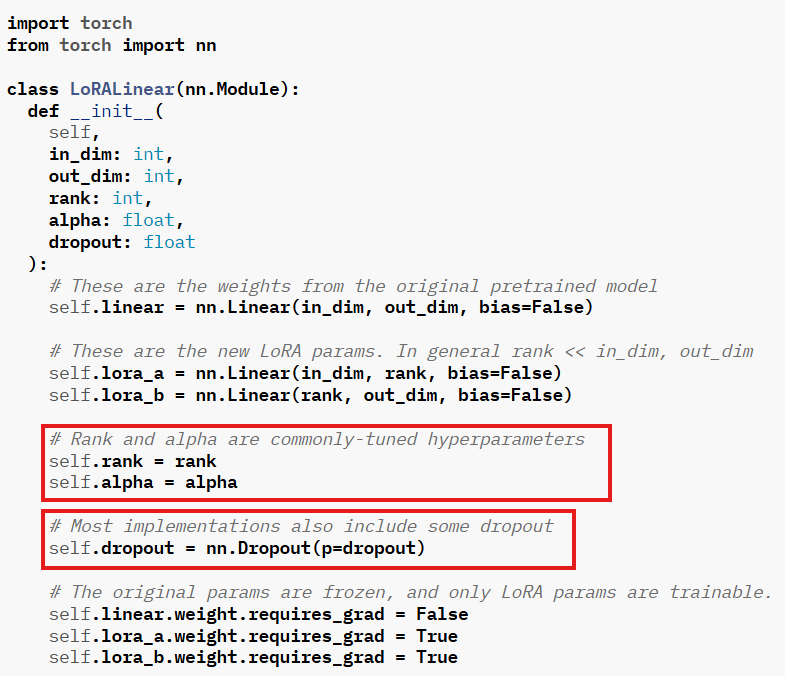
\includegraphics[width=1.0\textwidth]{images/lora.png}

\column{0.5\textwidth}

\begin{itemize}
    \item Fine-tuning of foundation models (e.g., LLMs) is very common these days, but the often used LORA \liturl{Hu et al. 2021}{https://arxiv.org/abs/2106.09685} also comes with several hyperparameters
    \item Also, these need to be tuned!
\end{itemize}
    
\end{columns}

\end{frame}
%-----------------------------------------------------------------------
%----------------------------------------------------------------------
\begin{frame}[c]{Code Generation: The Holy Grail!?}


\begin{columns}

\column{0.5\textwidth}

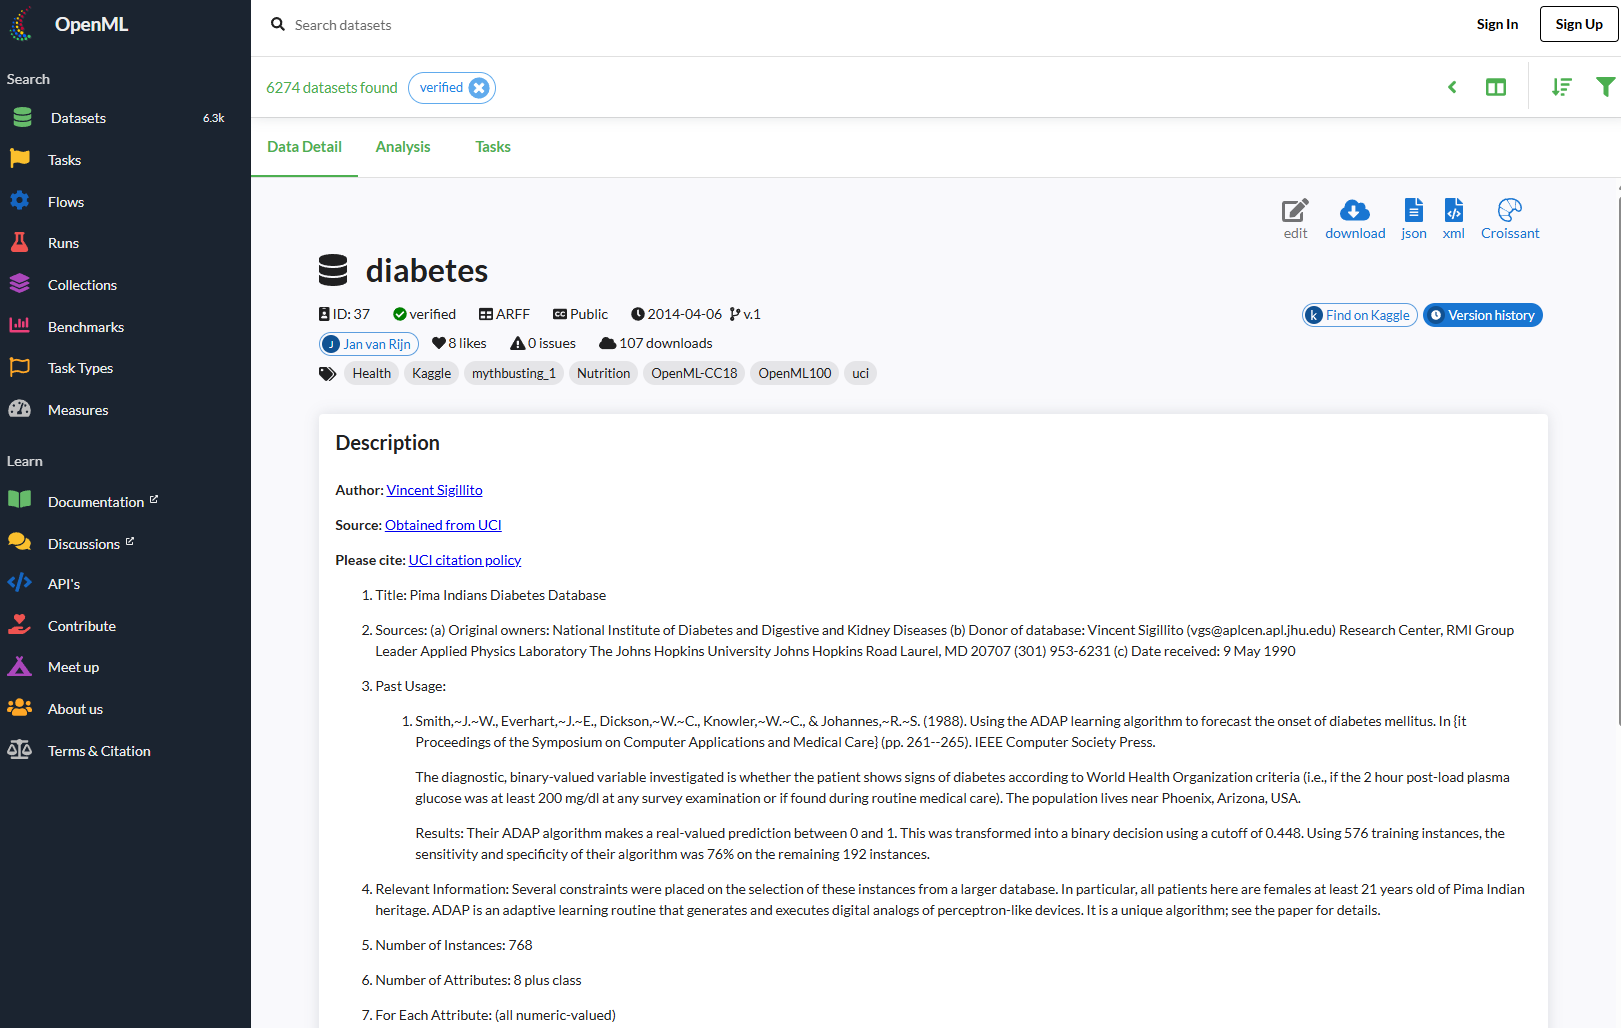
\includegraphics[width=1.0\textwidth]{images/openml_diabetes.png}

\column{0.5\textwidth}

\begin{itemize}
    \item Eventually, we would like to  get rid of manually written code entirely
    \item Code generation with LLMs~\liturl{Survey by Jiang et al.}{https://arxiv.org/abs/2406.00515} or Agentic systems \liturl{Survey by Plaat et al}{https://arxiv.org/abs/2503.23037} are a step in this direction
    \begin{itemize}
        \item \alert{Note}: As of the beginning of 2026, LLMs are not strong enough to do it on their own but need to employ existing (AutoML) tools to do a good job
    \end{itemize}
\end{itemize}
    
\end{columns}

\end{frame}
%-----------------------------------------------------------------------

%----------------------------------------------------------------------
\begin{frame}{Summary} 

Most important insights from this video:

\begin{enumerate}
    \item We strive for ML approaches that can learn on their own given data (``without being explicitly programmed'')
    \item In practice, ML workflows can be adapted to new (downstream) tasks via, e.g.,
    \begin{itemize}
        \item Hyperparameters (both for (pre-)training and fine-tuning)
        \item Architecture design
        \item Data preprocessing
        \item \ldots~(and much more, as you will learn in upcoming sessions)
    \end{itemize}
    \item Depending on how you set these, your ML project can be a great success or, in the worst case, a complete failure!
    \item \alert{Important:} How do you make these decisions?
\end{enumerate}

$\leadsto$ AutoML is the solution to these problems!

\end{frame}

\end{document}
